\section{L06-Sistemi aperti}
\subsection{Sistema aperto}
\begin{center}
    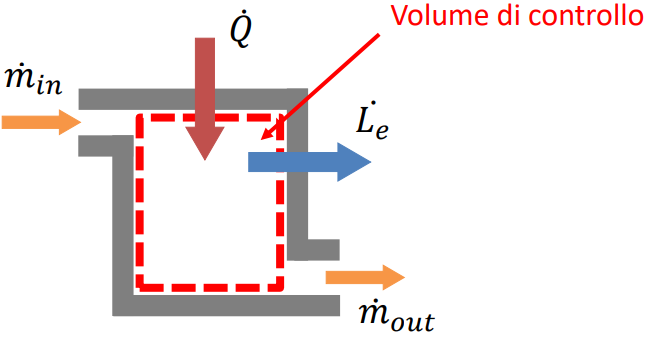
\includegraphics[height=3cm]{../L06/img1.PNG}
\end{center}
Un \textbf{sistema aperto} è un sistema dal quale può \textbf{uscire} ed \textbf{entrare massa}, per semplicità consideriamo una sola sezione di ingresso ed una sola sezione di uscita.\newline
\newline
Il sistema è percorso da \textbf{flussi monodimenisonali}:
\begin{itemize}
    \item sono presenti \textbf{condizioni di equilibrio} termodinamico sulle sezioni di \textbf{ingresso} e di \textbf{uscita};
    \item non viene fatta alcuna ipotesi in merito alla trasformazione termodinamica che il fluido subisce all'interno del sistema;
\end{itemize}
\ \newline
E' un \textbf{sistema fluente} e di conseguenza è necessario introdurre la \textbf{variabile tempo} ($t$) e di conseguenza i \textbf{flussi di massa}, \textbf{di energia}, \textbf{di entropia}, etc.
\[
    \dot{m} \;\;\;\;\; \dot{E}\;\;\;\;\;\dot{U}\;\;\;\;\;\dot{H}\;\;\;\;\;\dot{S}\;\;\;\;\;\dot{Q}\;\;\;\;\;\dot{L}
\]
\subsection{Equazioni di bilancio}
\subsubsection{Bilancio di mass}
Il bilancio di massa analizza la variazione di massa nel tempo del volume di controllo.
\[
    \frac{dM}{dt} = \sum_{k} \dot{m}_k^\leftarrow
\]
dove per $k$ si intendono le sezioni di passaggio, nel nostro caso 2, quella d'ingresso e quella d'uscita:
\[
    \frac{dM}{dt} = \dot{m}_i - \dot{m}_u
\]
\textbf{Equazione di continuità}:
\[
    \dot{m}=\rho w \Omega
\]
$\dot{m}$: portata;\newline
$\rho$: massa volumica;\newline
$w$: velocità media;\newline
$\Omega$: area della sezione di passaggio;
\subsubsection{Bilancio di energia}
\[
    \frac{dE}{dt}=\dot{E}^\leftarrow 
\]
L'\textbf{energia netta} entrante nel sistema:
\[
    \dot{E}^\leftarrow = \dot{Q}^\leftarrow - \dot{L}^\rightarrow + \sum_{k}\dot{E}_{m,k}^\leftarrow  + sorgenti
\]
$\dot{Q}^\leftarrow $: calore scambiato;\newline
$\dot{L}^\rightarrow $: lavoro scambiato;\newline
La sommatoria rappresenta lo scambio di energia associata al trasporto di massa per ogni sessione di passaggio, nel nostro caso 2, quelal d'ingresso e quella d'uscita;\newline
Le sorgenti sono le fonti di energia dovute a sorgenti (es. radiazioni, reazioni chimiche, etc.).\newline
\subsubsection{Calore scambiato}
\begin{itemize}
    \item Calore scambiato per unità di tempo attraverso le sezioni non attraversate dalla massa: $\dot{Q}^\leftarrow $;
    \item Calore scambiato per unità di tempo attraverso le sezioni attraversate dalla massa (ingresso e uscita): \textbf{trascurabile}
\end{itemize}
\subsubsection{Lavoro scambiato}
\begin{itemize}
    \item Lavoro scambiato per unità di tempo attraverso le sezioni non attraversate dalla massa: \textbf{lavoro di elica} $-\dot{L}_e^\rightarrow $ (che è la potenza meccanica che possiamo sfruttare);
    \item Lavoro scambiato per unità di tempo attraverso le sezioni attraversare dalla massa (ingresso e uscita): \textbf{lavoro di pulsione} $\dot{L}_P^\leftarrow $
\end{itemize}
\subsubsection{Lavoro di pulsione}
il \textbf{lavoro di pulsione} è il lavoro necessario per immettere ne lsistema la massa che il sistema scambia con l'esterno.
\begin{center}
    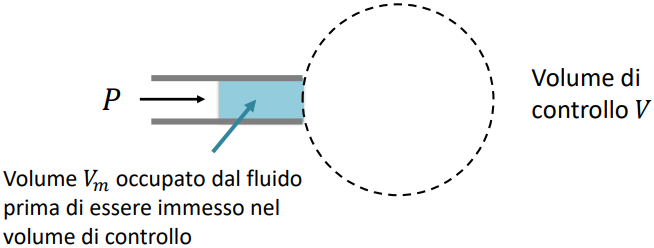
\includegraphics[height=3cm]{../L06/img2.PNG}
\end{center}
Si consideri un sistema $V + V_m$ occupato dalla massa $M + M_i$. Se si immette la massa $M_i$ nel volume $V$ il sistema complessivo subisce una variazione (riduzione) di volume mantenendo costante la massa.\newline
\newline
Questo è un sistema chiuso che scambia con l'esterno un lavoro $L_P^\leftarrow $:
\[
    L_P^\leftarrow  = - \int_{V-V_m}^{V}Pdv = P V_m
\]
dove $P$ è una costante. \newline
\newline
Per la \textbf{sessione di ingresso}:
\[
    L_P^\leftarrow  = M_i P v_i
\]
dove \newline
$M_i$: massa immessa nel sistema;\newline
$P$: pressione costante che agisce su $M_i$; \newline
$v_i$: volume specifico della sessione di ingresso.\newline
Allo stesso modo possiamo calcolarlo per la \textbf{sessione di uscita}.\newline
\newline
Questo termine di lavoro compare per ongi sezione di ingresso e di uscita della massa.
\subsubsection{Energia associata al trasporto di massa}
Nel valutare l'energia entrante nel sistema occorre tenere presente che la massa che attraversa la superficie di controllo trasporta con sè energia ($E_m$).\newline
\newline
Risulta somma delle energie associate ai flussi di massa (energia interna, energia potenziale ed energia cinetica):
\[
    \dot{E}_m = \sum_{k} \dot{m}_k^\leftarrow \left(u + gz + \frac{w^2}{2}\right)_k
\]
dove \newline
$k$: è il solito indice che itera su tutte le session idi scambio con l'esterno, nel nostro caso sono 2, quella di ingresso e quella d'uscita;\newline
$\dot{m}_k^\leftarrow $: portata; \newline
$u$: energia interna;\newline
$gz$: energia potenziale, con $g$ accellerazione gravitazionale e $z$ altitudine della sessione di passaggio;\newline
$\frac{w^2}{2}$: velocità media.
